\documentclass[11pt, a4paper, oneside]{article}

\usepackage{indentfirst}

% hifenização e outras especificações para português
\usepackage[portuguese]{babel}

% hiperligações
\usepackage{hyperref}
\hypersetup{colorlinks=true, urlcolor=blue, linkcolor=black}

% escrever acentos e coisas do género sem que o latex se desoriente
\usepackage[utf8]{inputenc}

% para ter imagens, depois define a directoria de imagens
\usepackage{graphicx}
\graphicspath{{./imagens/}}

\usepackage[labelformat=simple]{caption}
\usepackage[labelformat=empty]{subcaption}

% para ter a informação de quantas páginas tem o documento
\usepackage{lastpage}

% definir o cabeçalho e rodapé
\usepackage{fancyhdr}
\pagestyle{fancy}
\fancyhead[L]{\small{Processamento da Wikipédia}}
\fancyhead[R]{\small{Processamento de Linguagens}}

% ter enumerações alinhadas
\usepackage{enumitem}

% escrever algoritmos
\usepackage[algoruled]{algorithm2e}

% mais cores predefinidas
\usepackage[usenames,dvipsnames]{color}

% definir comandos especiais
\newcommand\doubleplus{+\kern-1.3ex+\kern0.8ex} %

\newcommand{\todo}[1] {\textcolor{BrickRed}{\begin{quote}#1\end{quote}}}

%\usepackage{listings}


%%%%%%%%%%%%%%%%%%%%%%%%%%%%%%%%%%%%%%%%%%%%%%
%% inicio do documento
\begin{document}
\title{Processamento da Wikipédia\\
\begin{normalsize}
Variante 1
\end{normalsize}}
\date{\today\\Universidade do Minho}
\author{
  Bruno Ferreira\\
  {\small A61055}\\
  \and
  Cláudia Oliveira\\
  {\small A60987}\\
  \and
  Vanessa Campos\\
  {\small A54801}\\
}

\maketitle

\begin{figure}[h]
\begin{center}

\includegraphics[width=0.4\linewidth]{logo}
\end{center}
\end{figure}


\begin{abstract}

  O presente trabalho foi desenvolvido no âmbito da Unidade Curricular de Processamento de Linguagens e tem como principal objectivo descrever o processo de desenvolvimento de um analisador léxico da \textit{Wikipédia}. Ao longo deste relatório iremos explicar as estruturas de dados que foram implementadas para o desenvolvimento deste trabalho, bem como todas as decisões que foram tomadas.

\end{abstract}
\newpage

\tableofcontents
\listoffigures 

\newpage
\section{Introdução}

Atualmente a \textit{Wikipédia} é a maior base de dados de conhecimento livre online e disponível em várias línguas. Neste contexto, pretende-se desenvolver um Processador de Texto, exportado da \textit{Wikipédia} e gerar a página html com os dados mais relevantes contidos nessa página, utilizando a ferramenta Flex. 
Com este trabalho foi necessário implementar Expressões Regulares de modo a retirar informação mais relevante num contexto enorme de informção, encontrando padrões que nos ajudem a descobrir o tipo de informação que estamos a procura e que é útil no contexto deste caso de estudo.


\newpage
\section{Desenvolvimento}

\subsection{Contextualização do Problema}

Flex é uma ferramenta para gerar automáticamente analisadores léxicos, isto é, programas que reconhecem padrões léxicos num texto. O Flex é uma evolução da ferramenta Lex, mas com a caraterística de ser mais rápido que este (Fast Lex). Lex foi desenvolvido por M.E. Lesk e E. Shmidt (Bell Laboratories - ATT) enquanto que o Flex é um produto da Free Software Foundation, Inc. Como são comumente distribuídos em sistemas Unix a sua documentação encontra-se na forma de manual pages para as entradas lex, flex e flexdoc. Ao contrário do programador que escreve manualmene um programa que realize a identificação de padrões numa entrada, o uso do Flex/Lex permite que sejam apenas especificados os padrões desejados e as ações necessárias para processá-los. Para que Flex/Lex reconheçam padrões no texto, tais padrões devem ser descritos através de expressões regulares. A ferramenta Flex é ótima para a realização deste trabalho uma vez que nos permite analisar o contéudo específico, através de expressões regulares de determinada informação de texto.

\subsection{Processamento da \textit{Wikipédia}}
Neste primeiro trabalho de Processamento de Linguagens foi-nos proposto escolher um tema a escolha, de vários enunciados propostos. Após uma análise cuidada  de cada um deles o nosso grupo optou por escolher o tema de Processamento da \textit{Wikipédia}. Esta escolha reflete-se pelo grande impacto que a \textit{Wikipédia} tem no nosso dia-a-dia e é a principal enciclopédia livre com mais utilizadores. 
O objectivo deste enunciado é criar um programa utilizando a ferramenta Flex que analise o contéudo de uma página XML da \textit{Wikipédia}, e que retire as informações relevantes dessa página como:
\begin{itemize}
\item título,
\item autor.
\item data
\item n.º de links internos
\item n.º de links externos
\item n.º de secções 
\end{itemize}
e criar uma página HTML (para cada página XML) com essas informações. Para isso é necessário exportar uma ou mais páginas usando o \textit{Special Export} disponível em \textbf{http://pt.wikipedia.org/wiki/Especial:Exportar (ou \\http://en.wikipedia.org/wiki/Special:Export} para a versão inglesa.
\newpage

\subsection{Enunciado}

De uma maneira geral, para teste trabalho pretende-se desenvolver os seguintes pontos:
\begin{itemize}
\item Especificar padrões de frases que se quer encontrar no texto fonte através de ERs.
\item Identificar as acções semânticas a realizar como reação ao reconhecimento de cada um desses padrões
\item Identificar estruturas de dados globais que possa eventualmente precisar para armazenar temporariamente a informação que se vai extraindo ou que se vai construindo à medida que o processamento avança.
\item Desenvolver um Processador de Texto para fazer reconhecimento dos padrões identificados e proceder à transformação pretendida, com recurso do Flex.
\end{itemize}

\subsection{Descrição do Problema}

Usando o \textbf{Especial Export} pretende-se exportar o contéudo da \textit{Wikipédia} e com o recurso do Flex implementar um processador de texto que deverá produzir, por cada página extraída do ficheiro XML, uma página \textbf{html} com as seguintes informações:

\begin{itemize}
\item Título
\item Autor da última revisão
\item Data da última revisão
\item Número de links internos, e explicitar quais.
\item Número de links externos, e explicitar quais.
\item Número de seções, e explicitar quais.
\item Opcional: mostrar na página \textit{html} o contéudo original do artigo.
\end{itemize}

\newpage

\subsection{Desenvolvimento do Programa}

\subsubsection{Estrutura de Dados}

Após termos analisado o ficheiro XML da \textit{Wikipédia} verificou-se que era necessário estruturar a informação encontrada nesses ficheiros. Essa informação é guardada em estruturas de dados que aqui vão ser expostas e explicadas. 

Primeiramente, vamos apresentar a estrutura de dados que armazena a informação das páginas.
\begin{figure}[h]
\begin{center}
\includegraphics[width=0.9\linewidth]{paginas}
\caption{Estrutura de Dados de Páginas}
\end{center}
\end{figure}


Como podemos verificar esta estrutura é uma lista-ligada que armazena a informação das páginas.


Para armazenar a informação dos componentes de cada página do XML, foi criado a seguinte estrutura de dados: \\
\begin{figure}[h]
\begin{center}
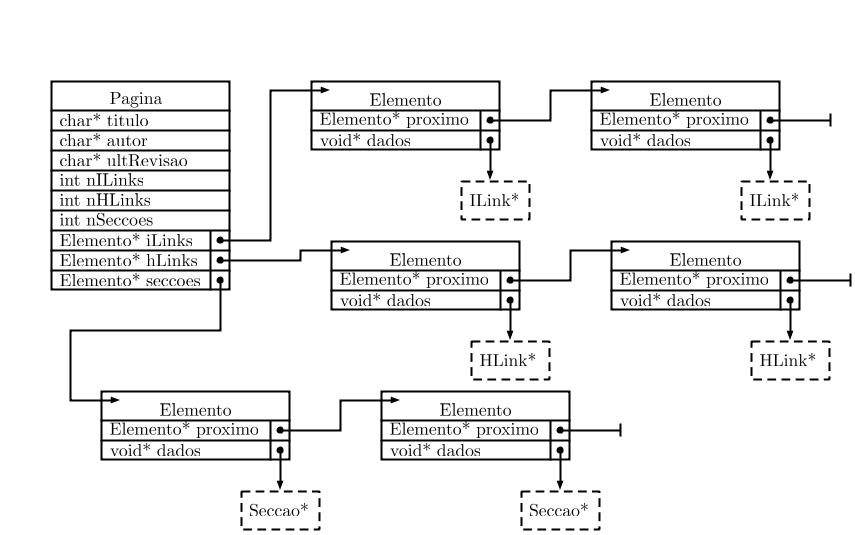
\includegraphics[width=0.9\linewidth]{pagina}
\caption{Estrutura de Dados de Página}
\end{center}
\end{figure}

Cada página consiste numa estrutura com a informação relativa à mesma, como titulo, autor, ultRevisao, mas também existem apontadores para outras listas-ligadas como a lista de links internos, links externos e secções.


Esses campos armazenam a seguinte informação:
\begin{itemize}

\item \textit{titulo} guarda o título do documento \textit{Wikipédia};
\item \textit{autor} guarda o autor da página;
\item \textit{ultRevisao} guarda a data da última revisão;
\item \textit{nILinks} guarda o número de links internos encontrados;
\item \textit{nHLinks} guarda o número de links externos encontrados;
\item \textit{nSeccões} guarda o número de secções encontradas;
\item \textit{iLikins} é o apontador para a estrutura Elemento, que guarda a informação dos links internos;
\item \textit{hLinks} é o apontador para a estrutura Elemento, que guarda a informação dos links externos;
\item \textit{seccoes} é apontador para a estrutura Elemento, que guarda a informação das secções da página;



\newpage
\end{itemize}
\subsubsection{Flex e Expressões Regulares}

Nesta secção iremos fazer uma abordagem as Expressões Regulares que foram desenvolvidas no contexto da resolução deste projecto. Utilizaram-se as seguintes condições de contexto:

\begin{verbatim}
%x page
%x title
%x revision
%x timestamp
%x contributor
%x username
%x text

%x ilink1
%x ilink2
%x ilink3
%x ilink4
%x hlink1
%x hlink2
%x head1
%x head2
%x head3
%x head4
%x head5
%x head6


\end{verbatim}

A cada uma das expressões regulares desenvolvidas neste projeto será feito uma breve descrição de cada uma delas, de modo a explicar a implementação do flex.

Começando por explicar as primeiras expressões regulares que foram implementadas: 

\begin{itemize}
\item 
\begin{verbatim}
"<page>"            {pag = pagina_create();
                     BEGIN page;
                    }
<page>"</page>"     {BEGIN 0;
                     paginas_add(paginas, pag);
                    }
\end{verbatim}
\end{itemize}
Aqui é guardado o início e o fim da página da leitura do ficheiro XML. Quando se encontra a tag \begin{math}<page>\end{math} inicia o estado page. Por outro lado, quando encontra \begin{math}</page>\end{math}, volta ao estado inicial. 
\\A função \begin{math}pagina\_create()\end{math} premite inicializar a estrutrua de dados que é uma página.
\\ A função \begin{math}paginas_add\end{math} adiciona uma nova página à lista ligada de páginas.

\begin{verbatim}

<page>"<title>"     BEGIN title;
<page>"<revision>"  BEGIN revision;
<title>"</title>"   BEGIN page;
<title>[^<]*        pagina_set_titulo(pag,yytext);

\end{verbatim}

Quando se está no estado page e é encontrada a tag \begin{math}<title>\end{math}, inicia-se o estado título e é apanhada o texto que se encontra dentro dessa tag até encontrar a \begin{math}</title>\end{math}, e guarda essa informação.


\begin{verbatim}
<page>"<revision>"  BEGIN revision;
<revision>"<timestamp>"    BEGIN timestamp;
<revision>"<contributor>"  BEGIN contributor;
<revision>"</revision>"    BEGIN page;
<revision>\<text.*?\>      BEGIN text;
\end{verbatim}


No caso de estarmos no estado page e é encontrado uma tag \begin{math}<revison>\end{math} esta indica quando foi feita a revisão à página. Depois entrar no estado \begin{math}<revison>\end{math} onde pode encontrar quatro estados: timestamp, contributor, page e text.

No caso de encontrar o timestamp:
\begin{verbatim}
<timestamp>"</timestamp>"  BEGIN revision;
<timestamp>[^<]*           pagina_set_ultimaRevisao(pag, yytext);
\end{verbatim}

A tag timestamp dá informação relativa à data e à horada da última revisão efectuada à página.
Quando se encontra a tag \begin{math}</timestamp>\end{math}  volta-se a tag revision, mas  temos também a função\begin{math}pagina\_set\_ultimaRevisao(Pagina* p, char* str)\end{math} que vai preencher na estrutura o campo ultimaRev com a informação relativa a esta tag.


No caso de encontrar o contributor:
\begin{verbatim}
<contributor>"<username>"      BEGIN username;
<contributor>"</contributor>"  BEGIN revision;

\end{verbatim}
A tag \begin{math}<contributor>\end{math} é onde se pode encontrar a definição do autor da página. 
Quando dentro da tag contributor é apanhada pelo flex o texto "<username>" passa-se a tag  \begin{math}<username>\end{math}.
Se a tag \begin{math}</contributor>\end{math} é a panhada signifia que chegou ao fim a informação do colaborador da página, onde depois voltamos para o estado anterior que neste caso e a revision. 

No caso de encontrar o  username:
\begin{verbatim}
<username>"</username>"    BEGIN contributor;
<username>[^<]*            pagina_set_autor(pag, yytext);
\end{verbatim}
A tag \begin{math}<username>\end{math} é onde está definido quem é o autor da página. Para armazenar o autor na página tem-se a função\begin{math}pagina\_set\_autor(Pagina* p, char* str)\end{math} que vai preencher o campo autor na estrutura da página.

<text>"</text>"     BEGIN revision;
Quando estamos neste caso significa que se está a processar o caso em que nós encontramos o fim do texto da página.


No caso de encontrarmos as seguintes expressões, significa que todo o tipo de cabeçalhos da wikipédia estão a ser apanhados. Iremos aboradar mais abaixo o que significa cada um deles.

\begin{verbatim}

<text>\n\=          BEGIN head1;
<text>\n\={2}       BEGIN head2;
<text>\n\={3}       BEGIN head3;
<text>\n\={4}       BEGIN head4;
<text>\n\={5}       BEGIN head5;
<text>\n\={6}       BEGIN head6;
\end{verbatim}

No caso de encontrar no texto "[[File:" ou "[[Image:" não é feita qualquer acção de tratamento por parte do flex. No entanto quando temos "[[" significa que foi apanhado um internal link, se aparecer "[" então foi encontrado um hyper link.

\begin{verbatim}
<text>"[[File:"     ;
<text>"[[Image:"    ;
<text>"[[":?        BEGIN ilink1;
<text>"["           BEGIN hlink1;
\end{verbatim}

No caso dos links externos, apanha-se o [, de seguida apanha o URI até encontrar um ] ou um espaço. Se encontrar um espaço tudo o que venha até a ]  é o texto que se vai filtrar.
\begin{verbatim}
<hlink1>[^\ \]]+    {/*leu o uri*/
                     hlink = hlink_create();
                     pagina_add_hlink(pag, hlink);
                     hlink_set_uri(hlink, yytext);
                     BEGIN hlink2;
                    }
\end{verbatim}

Quando é  encontrado pelo flex a expressão exposta em cima, tem-se que é inicializado um hlink através de \begin{math} hlink\_create() \end{math}, depois é adicionado a lista de links da página  \begin{math} paginas\_add(Elemento* ps, Pagina* p)\end{math}. Por fim  é necessário indicar qual o uri que o link tem, usando a função  \begin{math} hlink\_set\_uri(HLink* hlink, char* str)\end{math}.
No entanto é necessário ver se o hlink possui mais informação dai no fim ser chamado o hlink2.


\begin{verbatim}
<hlink2>\ [^\]]+    hlink_set_texto(hlink, yytext+1);
<hlink2>\]          BEGIN text;

\end{verbatim}

O hlink2 é onde vai ver onde é que o hlink acaba, pois pode dar-se o caso de o hlink possuir texto para substituir o hlink, e para isso existe a seguinte expressão para apanhar o resto do texto. Depois de apanhado todo o texto até ao "]]" para adicionar ao hlink o resto da informação existe a função \begin{math} hlink\_set\_texto(HLink* hlink, char* str) \end{math} para isso.

Nas descrições que se seguem, vão ser descritos como é que os links internos das páginas são apanhados e tratados.
Quando se fala de links, existem vários tipos que firam definidos como sendo:
\begin{itemize}
\item special;
\item texto;
\item parênteses;
\item virgula;
\item apresentar;
\item resto;
\end{itemize}


Vai ser explicado como é que cada tipo é apanhado.

\begin{verbatim}
<ilink1>[a-zA-Z]+:[^\]\(,\|]+  { ilink = ilink_create();
                       ilink_set_especial(ilink, yytext); 
                       BEGIN ilink2;}
\end{verbatim}


Quando é apanhada a expressão regular acima significa que foi apanhado um link que é formado como sendo \begin{math}[[Category:Salts]]\end{math} depois o link apanhar vai inicializar a estrutura de links internos \begin{math} ilink\_create() \end{math} e depois vai definir que existe um link e vai armazenar o texto relativo ao link.

\begin{verbatim}
<ilink1>[^\]\(,\|]+    { ilink = ilink_create();
                       ilink_set_texto(ilink, yytext);
                       BEGIN ilink2;}
\end{verbatim}
Esta expressão regular apanha um link internos que seja da seguinte forma :\begin{math}[[Salts]]\end{math}, onde o que se encontra dentro do parênteses é o link em si. Depois de termos o link definido chamamos as função \begin{math} ilink\_create() \end{math} para inicialização do link e  \begin{math}ilink\_set\_texto(ilink, yytext)\end{math} para guardar o link na estrutura de links internos (Ilink).


\begin{verbatim}

<ilink2,ilink3>\]      {BEGIN ilink4;}
\end{verbatim}
Este caso existe para que caso o flex se encontre na condição de contexto \begin{math}<ilink2>\end{math} ou \begin{math}<ilink3>\end{math} e a seguir exista "]" o flex vai entrar na condiçãode contexto \begin{math}ilink4\end{math}




\begin{verbatim}
<ilink2>\|               {BEGIN ilink3;}
\end{verbatim}


Neste ponto significa que existe no link2 mais alguma coisa, isto é o link e do formato \begin{math}[[Crystallite|grain boundaries]]\end{math}, pois o link possui um pipe e para tratar o pipe o flex vai para a condição de contexto link3, onde depois vai analisar o resto do link. 


\begin{verbatim}
<ilink2>\([^\]\)\|]+\)\]  {yytext[ strlen(yytext)-1 ] = '\0';
                          ilink_set_parenteses(ilink, yytext);
                          BEGIN ilink4;}

\end{verbatim}

Neste caso está a ser apanhado um link que pode ter a seguinte estrutura \begin{math}[[Opacity (optics)]]\end{math}. Depois de termos o link,  transforma-se para numa string dai o '\\0'.
Após termos o link vai-se guardar o texto do yytext na estrutura dos links internos (Ilink), mas como não sabemos se o link pode ter mais informação o flex vai a condição de contexto ilink4 "fazer" essa verificação. 

\begin{verbatim}
<ilink2>\([^\]\)\|]+\)\|  {yytext[ strlen(yytext)-1 ] = '\0';
                         ilink_set_parenteses(ilink, yytext);
                         BEGIN ilink3;}
\end{verbatim}
Quando existe uma expressão regular deste género significa que o link pode ter o seguinte formato \begin{math}[[Opacity ((optics))|]]\end{math} que quando analisado em profundo concluiu-se que o link é válido por isso era necessário ver os parênteses que o link "trazia".
Depois de a totalidade do link ser capturada usou-se a função para o armazenar na estrutura definida para os ilinks.

\begin{verbatim}
<ilink2>\([^\]\)\|]+\|   {yytext[ strlen(yytext)-1 ] = '\0';
                         ilink_set_parenteses(ilink, yytext);
                         BEGIN ilink3;}
\end{verbatim}

Esta expressão serve para apanhar os links internos onde a sua estrutura pode ter a forma \begin{math}[[Opacity ((optics|]]\end{math}, por isso era necessário garantir que os parênteses eram apanhados, pois o link é válido. 
Depois do link apanhado é tratado com a função \begin{math} ilink\_set\_parenteses(ilink, yytext)\end{math} que adiciona o link à estrutura de dados dos ilinks, como o link esta guardado o flex vai para ilink3 para continuar o tratamento dos links.

\begin{verbatim}
<ilink2>\([^\]\)\|]+\]   {yytext[ strlen(yytext)-1 ] = '\0';
                        ilink_set_parenteses(ilink, yytext);
                        BEGIN ilink4;}
\end{verbatim}
Por fim quando o flex entra nesta condição de contexto, significa que foi encontrado um link \begin{math}([[Opacity (optics)|texto]])\end{math} em que temos o link, mas esse link possui um texto para a substituição do endereço do link.
Neste caso, o link possui mais informação, dai o BEGIN ilink4, pois é necessário apanhar o texto que existe depois dos parênteses.

\begin{verbatim}
<ilink2>,[^\]\|]*\]    {yytext[ strlen(yytext)-1 ] = '\0';
                       ilink_set_virgula(ilink, yytext);
                       BEGIN ilink4;}
\end{verbatim}
%A este caso existe um link \begin{math}[[Opacity, Não via ser apanhar]\end{math} em que o que se encontra a seguir a virgula não é apanhado, o que é apenas apanhado é o que neste exemplo é o "Opacity".

\begin{verbatim}
<ilink2>,[^\]\|]*\|    {yytext[ strlen(yytext)-1 ] = '\0';
                       ilink_set_virgula(ilink, yytext);
                       BEGIN ilink3;}
\end{verbatim}
%Quando a expressão regular é apanhada significa que o link em causa tem a forma de: \begin{math}[[Opacity, Não via ser apanhar| texto]] \end{math}, onde o texto que se encontra a seguir ao pipe vais substituir o texto que apresentado para esse link.

\begin{verbatim}
<ilink3>[^\]]*\]       {yytext[ strlen(yytext)-1 ] = '\0';
                       ilink_set_apresentar(ilink, yytext);
                       BEGIN ilink4;}
\end{verbatim}
Esta expressão é onde os links são apanhados para depois serem convidos em strings e armazenados na estrutura de dados dos ilinks.

\begin{verbatim}
<ilink4>\][a-zA-Z]*    {ilink_set_resto(ilink, yytext+1);
                       pagina_add_ilink(pag, ilink);
                       BEGIN text;}
\end{verbatim}

Nesta expressão vai apanhar o resto do texto do link, e como o link quando aqui já esta na sua totalidade pode-se então guardar a estrutura dos links na página correspondente.


\begin{verbatim}
<ilink1,ilink2,ilink3>.             ;
\end{verbatim}
Esta expressão só é apanhada apara que os links que não entrem expressões acima sejam filtrados pelo flex. 



\begin{verbatim}
<head1>[^\=]+  pagina_add_seccao(pag, seccao_create(yytext, 1));
<head2>[^\=]+  pagina_add_seccao(pag, seccao_create(yytext, 2));
<head3>[^\=]+  pagina_add_seccao(pag, seccao_create(yytext, 3));
<head4>[^\=]+  pagina_add_seccao(pag, seccao_create(yytext, 4));
<head5>[^\=]+  pagina_add_seccao(pag, seccao_create(yytext, 5));
<head6>[^\=]+  pagina_add_seccao(pag, seccao_create(yytext, 6));
\end{verbatim}
As expressões que se encontram em cima são as responsáveis para fechar a expressão que permite apanhar o headers, e chama a respetiva função que os vais guardar na estrutura de dados das secções. Os headers são definidos de 1 a 6. em que cada função esta definida para um próprio header. 

\begin{verbatim}
<head1>\={1}                        BEGIN text;
<head2>\={2}                        BEGIN text;
<head3>\={3}                        BEGIN text;
<head4>\={4}                        BEGIN text;
<head5>\={5}                        BEGIN text;
<head6>\={4}                        BEGIN text;

\end{verbatim}
Já as estas expressões servem para depois de os headers serem apanhados, voltar a text.

\newpage
\section{Conclusão}

Após concluir todo o desenvolvimento deste projecto é fácil fazer um balanço de todo este precurso. Para além de ter sido um desafio implementar um programa de processamento da \textit{Wikipédia}, foi também aliciante concluir todo o trabalho.
Ao longo do desenvolvimento do projeto o grupo desenvolveu competências em diversas ferramentas como C,HTML, XML, Flex, etc, que anteriormente eram poucas e até mesmo desconhecidas em alguns dos casos. 
A utilização do Flex permitiu filtrar a informação mais relevante da página da \textit{Wikipédia} através do uso de expressões regulares. 
\newpage
\section{Apêndices - Especificação do Flex}

\subsection{Código escrito em flex}
\begin{verbatim}
/* Not Another Wikipedia Parser
%option debug*/

%x page
%x title
%x revision
%x timestamp
%x contributor
%x username
%x text

%x ilink1
%x ilink2
%x ilink3
%x ilink4
%x hlink1
%x hlink2
%x head1
%x head2
%x head3
%x head4
%x head5
%x head6


%{
#include "paginas.h"
#include "pagina.h"
#include "ilink.h"
#include "hlink.h"

ILink* ilink = NULL;
HLink* hlink = NULL;
Pagina* pag = NULL;
Elemento* paginas = NULL;

%}
%%
    paginas = paginas_create();

"<page>"            {pag = pagina_create();
                     BEGIN page;
                    }
<page>"</page>"     {BEGIN 0;
                     paginas_add(paginas, pag);
                    }

<page>"<title>"     BEGIN title;

<page>"<revision>"  BEGIN revision;

<title>"</title>"   BEGIN page;

<title>[^<]*        pagina_set_titulo(pag,yytext);

<revision>"<timestamp>"    BEGIN timestamp;
<revision>"<contributor>"  BEGIN contributor;
<revision>"</revision>"    BEGIN page;
<revision>\<text.*?\>      BEGIN text;

<timestamp>"</timestamp>"  BEGIN revision;
<timestamp>[^<]*           pagina_set_ultimaRevisao(pag, yytext);

<contributor>"<username>"      BEGIN username;
<contributor>"</contributor>"  BEGIN revision;

<username>"</username>"    BEGIN contributor;
<username>[^<]*            pagina_set_autor(pag, yytext);

<text>"</text>"     BEGIN revision;

<text>\n\=          BEGIN head1;
<text>\n\={2}       BEGIN head2;
<text>\n\={3}       BEGIN head3;
<text>\n\={4}       BEGIN head4;
<text>\n\={5}       BEGIN head5;
<text>\n\={6}       BEGIN head6;
<text>"[[File:"     ;/*ignorar [[ caso sejam ficheiros*/
<text>"[[Image:"    ;/*ignorar [[ caso sejam imagens*/
<text>"[[":?        BEGIN ilink1;
<text>"["           BEGIN hlink1;

<hlink1>[^\ \]]+    {/*leu o uri*/
                     hlink = hlink_create();
                     pagina_add_hlink(pag, hlink);
                     hlink_set_uri(hlink, yytext);
                     BEGIN hlink2;
                    }
<hlink2>\ [^\]]+    hlink_set_texto(hlink, yytext+1);
<hlink2>\]          BEGIN text;

<ilink1>[a-zA-Z]+:[^\]\(,\|]+       {/*ABCJ */
                                     ilink = ilink_create();
                                     ilink_set_especial(ilink, yytext);
                                     BEGIN ilink2;                                    }

<ilink1>[^\]\(,\|]+                 {/*ABC  */
                                     ilink = ilink_create();
                                     ilink_set_texto(ilink, yytext);
                                     BEGIN ilink2;
                                    }

<ilink2,ilink3>\]                   {/*D    */
                                     BEGIN ilink4;
                                    }

<ilink2>\|                          {/*H    */
                                     BEGIN ilink3;
                                    }

<ilink2>\([^\]\)\|]+\)\]            {/*EFGD */
                                     yytext[ strlen(yytext)-1 ] = '\0';
                                     ilink_set_parenteses(ilink, yytext);
                                     BEGIN ilink4;
                                    }

<ilink2>\([^\]\)\|]+\)\|            {/*EFGH */
                                     yytext[ strlen(yytext)-1 ] = '\0';
                                     ilink_set_parenteses(ilink, yytext);
                                     BEGIN ilink3;
                                    }

<ilink2>\([^\]\)\|]+\|              {/*EFH  */
                                     yytext[ strlen(yytext)-1 ] = '\0';
                                     // deve adicionar ao texto, 
                                     e nao meter em parenteses
                                     ilink_set_parenteses(ilink, yytext);
                                     BEGIN ilink3;
                                    }

<ilink2>\([^\]\)\|]+\]              {/*EFD  */
                                     yytext[ strlen(yytext)-1 ] = '\0';
                                     // deve adicionar ao texto, 
                                     e nao meter em parenteses
                                     ilink_set_parenteses(ilink, yytext);
                                     BEGIN ilink4;
                                    }

<ilink2>,[^\]\|]*\]                 {/*KMD  */
                                     yytext[ strlen(yytext)-1 ] = '\0';
                                     ilink_set_virgula(ilink, yytext);
                                     BEGIN ilink4;
                                    }

<ilink2>,[^\]\|]*\|                 {/*KMH  */
                                     yytext[ strlen(yytext)-1 ] = '\0';
                                     ilink_set_virgula(ilink, yytext);
                                     BEGIN ilink3;
                                    }

<ilink3>[^\]]*\]                    {/*ID   */
                                     yytext[ strlen(yytext)-1 ] = '\0';
                                     ilink_set_apresentar(ilink, yytext);
                                     BEGIN ilink4;
                                    }

<ilink4>\][a-zA-Z]*                 {/*L    */
                                     ilink_set_resto(ilink, yytext+1);
                                     //ilink_print(ilink);
                                     pagina_add_ilink(pag, ilink);
                                     BEGIN text;
                                    }

<ilink1,ilink2,ilink3>.             ;

<head1>[^\=]+                       pagina_add_seccao(pag, 
                                    seccao_create(yytext, 1));
<head2>[^\=]+                       pagina_add_seccao(pag, 
                                    seccao_create(yytext, 2));
<head3>[^\=]+                       pagina_add_seccao(pag, 
                                    seccao_create(yytext, 3));
<head4>[^\=]+                       pagina_add_seccao(pag, 
                                    seccao_create(yytext, 4));
<head5>[^\=]+                       pagina_add_seccao
                                    (pag, seccao_create(yytext, 5));
<head6>[^\=]+                       pagina_add_seccao
                                    (pag, seccao_create(yytext, 6));
<head1>\={1}                        BEGIN text;
<head2>\={2}                        BEGIN text;
<head3>\={3}                        BEGIN text;
<head4>\={4}                        BEGIN text;
<head5>\={5}                        BEGIN text;
<head6>\={4}                        BEGIN text;

<*>. ;
<*>\n ;
%%
int yywrap(){
    // escrever todas as infos
    paginas_print(paginas);

    // os destroys todos

    return 1;
}
\end{verbatim}
\newpage

\subsection{Cógido do Ficheiro Página.c}
\begin{verbatim}
#include "pagina.h"

#include <stdio.h>
#include <stdlib.h>
#include <string.h>

// -1 se str1 <  str2
//  0 se str1 == str2
// +1 se str1 >  str2
int myStrCmp( char* str1, char* str2 ){
    if( !str1 && !str2 )
        return 0;
    
    if( !str1 && str2)
        return -1;
    
    if( str1 && !str2)
        return 1;
    

    //percorrer todos os iguais
    while(*str1 == *str2 && *str1 != '\0' && *str2 != '\0'){
        str1++;
        str2++;
    }
    
    if( *str1 < *str2 )
        return -1;
    
    if( *str1 > *str2 )
        return 1;
    

    // caso em que são iguais
    return 0;
}

void printTitulos(Elemento* ps){
    Elemento* itr = ps;
    
    // ordenado pelo titulo
    fprintf(stderr, "PS: ");
    while( itr ){
        fprintf(stderr, "%s -> ", ((Pagina*)(itr->dados))->titulo);
        itr = itr->proximo;
    }
    fprintf(stderr, "\n");
}

Elemento* paginas_create(){
    Elemento* paginas = (Elemento*) malloc(sizeof(Elemento));

    paginas->proximo = NULL;
    paginas->dados = NULL;

    return paginas;
}

void paginas_add(Elemento* ps, Pagina* p){
    if( ps->dados == NULL ){
        // primeira pagina
        ps->dados = p;
        return;
    }
    
    //printTitulos(ps);
    
    Elemento* e = (Elemento*) malloc( sizeof(Elemento));

    e->dados = p;
    e->proximo= NULL;

    Elemento* itr = ps;
    
    // inserir ordenado pelo titulo
    while( itr->proximo != NULL && 
    myStrCmp(((Pagina*)(itr->dados))->titulo, p->titulo) < 0)
        itr = itr->proximo;
    

    e->proximo = itr->proximo;
    itr->proximo = e;

    void* dadosSwap;
    if( myStrCmp(((Pagina*)(itr->dados))->titulo, p->titulo) > 0 ){
        dadosSwap = e->dados;
        e->dados = itr->dados;
        itr->dados = dadosSwap;
    }
        
}

void paginas_destroy(Elemento** paginas){
    if( *paginas == NULL )
        return;
    
    pagina_destroy( (Pagina**) &((*paginas)->dados) );

    paginas_destroy( &((*paginas)->proximo) );
    
    free(*paginas);
}

void paginas_print(Elemento* paginas){
    Elemento* itr;
    Pagina* pActual;
    int i;
    
    // head
    printf("<html><head><meta http-equiv=\"Content-Type
    \" content=\"text/html;charset=UTF-8\"><link rel=
    \"stylesheet\" type=\"text/css\" 
    href=\"http://bootswatch.com/cosmo/bootstrap.css\
    "><title>Processamento de Linguagens</title></head>");
    
    // inicio do body
    printf("<body style=\"width:90%%; margin-left: auto; 
    margin-right: auto; margin-top: 25px;\"><a name=\"top\"></a>");
    printf("<div class=\"panel panel-default\"><div class=
    \"panel-body\"><h2><b>N</b>ot <b>A</b>nother <b>W</b>
    ikipedia <b>P</b>arser<img src=\"http://corpora.di.uminho.pt/
    linguateca/pagina_linguateca/logoUM.jpg\" alt=\
    "Escola de Engenharia da Universidade do Minho\" 
    width=\"150\" height=\"75\" align=\"top;\" style=\
    "float:right;position:relative;bottom:20px\">
    </h2></div></div><div class=\"panel panel-default\">
    <div class=\"panel-heading\"><h3>Índice de páginas
    </h3></div><div class=\"panel-body\"><dl>");
    
    // lista de paginas
    i=0;
    itr = paginas;
    while( itr ){
        pActual = (Pagina*) itr->dados;
        pActual->indice = i++;
        printf("<dt><a href=\"#pagina%d\">%s</a></dt>\n", 
        pActual->indice, pActual->titulo);
        //pagina_print( (Pagina*)itr->dados);
        itr = itr->proximo;
    }
    printf("</dl></div></div>");
    
    // imprimir as páginas
    itr = paginas;
    while( itr ){
        pagina_print( (Pagina*)itr->dados);
        itr = itr->proximo;
    }
    printf("</dl></div></div>");
    
    
    // terminar o HTML
    printf("</body></html>\n\n");
}
\end{verbatim}
\newpage
\subsection{Código do ficheiro pagina.c}
\begin{verbatim}


#include <stdlib.h>
#include <stdio.h>
#include <string.h>

#include "pagina.h"

// cria uma nova página
Pagina* pagina_create(){
    Pagina* p = (Pagina*) malloc(sizeof(Pagina));

    p->titulo = NULL;
    p->ultimaRev = NULL;
    p->autor = NULL;

    p->iLinks = NULL;
    p->nILinks = 0;

    p->hLinks = NULL;
    p->nHLinks = 0;

    p->seccoes = NULL;
    p->nSeccoes = 0;

    p->indice = -1;

    return p;
}

void pagina_set_titulo(Pagina* p, char* str){
    //recebe:
    //texto da pagina

    p->titulo = (char*) malloc( strlen(str)+1 );
    strcpy( p->titulo, str);
}

// insere o autor
void pagina_set_autor(Pagina* p, char* str){
    p->autor = (char*) malloc( strlen(str)+1 );
    strcpy( p->autor, str);
}

// insere o ultimaRevisao
void pagina_set_ultimaRevisao(Pagina* p, char* str){
    p->ultimaRev = (char*) malloc( strlen(str)+1 );
    str[10] = str[19] = ' ';
    strcpy( p->ultimaRev, str);
}

// destroi a página
void pagina_destroy(Pagina** pag){
    Pagina* p = *pag;

    free(p->titulo);
    free(p->ultimaRev);
    free(p->autor);

    // falta aqui a parte destruir os elementos das listas
    

    free(*pag);
}

void pagina_print(Pagina* p){
    Elemento* itr = NULL;
    int i;
    
    printf("<div class=\"panel panel-default\"><a name=
    \"pagina%d\"></a><div class=\"panel-heading\"><h1>%s</h1>
    <div style=\"width:100%%\"><button type=\"button\" class=
    \"btn btn-danger disabled\" align = 
    \"left\">Ultima alteração em %s por %s</button><a href=
    \"#top\"><button type=\"button\" class=\"btn btn-default\" 
    style =\"float:right\">&uarr;</button></a></div></div><div 
    class=\"panel-body\"><div class=\"subsection\" id=\"cont\">
    <h3>Secções (%d)</h3>\n", p->indice, p->titulo, p->ultimaRev, 
    p->autor, p->nSeccoes);

    // imprimir as seccões
    Seccao *seccao = NULL;
    for( itr=p->seccoes; itr; itr = itr->proximo ){
        seccao = itr->dados;
        seccao_print(seccao);
    }
    
    printf("</div><hr width=100%%><table class=\"table 
    table-striped \"><thead><tr class=\"info\"><th 
    style=\"width:50%%\" colspan=2>%d Links Externos
    </th></tr></thead><tbody>", p->nHLinks);
    
    itr = p->hLinks;
    for(i=0; i < p->nHLinks/2; i+=1){
        printf("<tr><td>");
        hlink_print((HLink*)itr->dados);

        itr = itr->proximo;
        printf("</td><td>");
        hlink_print((HLink*)itr->dados);
        printf("</td></tr>\n");

        itr = itr->proximo;
    }

    if( itr ){
        printf("<tr><td>");
        hlink_print((HLink*)itr->dados);
        printf("</td><td></td></tr>");
    }
    printf("</tbody></table>");


    printf("<hr width=100%%><table class=\
    "table table-striped\"><thead><tr class=\"info\">
    <th style=\"width:50%%\"colspan=2>%d Links Internos
    </th></tr></thead><tbody>", p->nILinks);

    itr = p->iLinks;
    for(i=0; i < p->nILinks/2; i+=1){
        printf("<tr><td>");
        ilink_print((ILink*)itr->dados);

        itr = itr->proximo;
        printf("</td><td>");
        ilink_print((ILink*)itr->dados);
        printf("</td></tr>\n");

        itr = itr->proximo;
    }

    if( itr ){
        printf("<tr><td>");
        ilink_print((ILink*)itr->dados);
        printf("</td><td></td></tr>");
    }
    
    printf("</tbody></table></div></div>");
}

void pagina_add_ilink(Pagina* pagina, ILink* linkinfo){
    Elemento* e = (Elemento*) malloc( sizeof(Elemento));

    e->dados = linkinfo;
    e->proximo= NULL;

    Elemento* itr = pagina->iLinks;
    pagina->nILinks++;
    
    // se ainda nao houver elementos na lista
    if( itr == NULL ){
        pagina->iLinks = e;
        return;
    }
    
    // se ja houver elementos, percorrer até ao ultimo e 
    //inserir
    while( itr->proximo != NULL )
        itr = itr->proximo;

    itr->proximo = e;
}

void pagina_add_seccao(Pagina* pagina, Seccao* seccao){
    Elemento* e = (Elemento*) malloc( sizeof(Elemento));

    e->dados = seccao;
    e->proximo= NULL;

    Elemento* itr = pagina->seccoes;
    pagina->nSeccoes++;
    
    // se ainda nao houver elementos na lista
    if( itr == NULL ){
        pagina->seccoes = e;
        return;
    }
    
    // se ja houver elementos, percorrer até ao ultimo e 
    //inserir
    while( itr->proximo != NULL )
        itr = itr->proximo;
    
    itr->proximo = e;
}


void pagina_add_hlink(Pagina* pagina, HLink* linkinfo){
    Elemento* e = (Elemento*) malloc( sizeof(Elemento));

    e->dados = linkinfo;
    e->proximo= NULL;

    Elemento* itr = pagina->hLinks;
    pagina->nHLinks++;
    
    // se ainda nao houver elementos na lista
    if( itr == NULL ){
        pagina->hLinks = e;
        return;
    }
    
    // se ja houver elementos, percorrer até ao ultimo e 
    //inserir
    while( itr->proximo != NULL )
        itr = itr->proximo;
    
    itr->proximo = e;
}

\end{verbatim}

\newpage
\subsection{Código do ficheiro ilink.c}
\begin{verbatim}
#include <stdlib.h>
#include <string.h>
#include <stdio.h>

#include "ilink.h"

static void string_replace(char* str, const char find, 
const char replace){
    if(!str) return;
    
    while(*str != '\0'){
        if(*str == find)
            *str = replace;
        str++;
    }
}

ILink* ilink_create(){
    ILink* ilink = (ILink*) malloc(sizeof(ILink));

    ilink->parenteses = NULL;
    ilink->texto = NULL;
    ilink->virgula = NULL;
    ilink->apresentar = NULL;
    ilink->resto = NULL;
    ilink->especial = NULL;

    return ilink;
}

void ilink_set_especial(ILink* ilink, char* str){
    
    //recebe coisas como:
    //help:texto da pagina
    
    char* especial = strtok(str, ":");
    char* texto = strtok(NULL, ":");

    ilink->especial = (char*) malloc( strlen(especial)+1 );
    strcpy( ilink->especial, especial );
    
    ilink->texto = (char*) malloc( strlen(texto)+1 );
    strcpy( ilink->texto, texto );
    string_replace(ilink->texto, ' ', '_');
}

void ilink_set_texto(ILink* ilink, char* str){
    //recebe:
    //texto da pagina

    ilink->texto = (char*) malloc( strlen(str)+1 );
    strcpy( ilink->texto, str);
    //string_replace(ilink->texto, ' ', '_');
}

void ilink_set_parenteses(ILink* ilink, char* str){

    //recebe:
    //(coisas entre parenteses)
    //(coisas que nao acabam com parenteses
    
    if( str[strlen(str)-1] == ')' ){
        ilink->parenteses = (char*) 
        malloc( strlen(str)+1 );
        strcpy( ilink->parenteses, str );
        string_replace(ilink->parenteses, ' ', '_');
    }else{
        //nao termina com parenteses e por isso é o 
        //segundo caso
        char* acumulador = (char*) malloc( strlen(str) 
        + strlen(ilink->texto) + 1 );
        acumulador[0] = '\0';
        strcat(acumulador, ilink->texto);
        strcat(acumulador, str);
        free( ilink->texto );
        ilink->texto = acumulador;
    }
}

void ilink_set_virgula(ILink* ilink, char* str){

    //recebe:
    //, coisas depois de uma virgula

    ilink->virgula = (char*) malloc( strlen(str)+1 );
    strcpy( ilink->virgula, str );
    string_replace(ilink->virgula, ' ', '_');
}

void ilink_set_apresentar(ILink* ilink, char* str){

    //recebe:
    //coisas que aparecerem depois do pipe
    //\ \t
    
    while(*str == ' ') //retirar espaços em 
                        //branco no início
        str++;

    ilink->apresentar = (char*) malloc( strlen(str)+1 );
    strcpy( ilink->apresentar, str );
}

void ilink_set_resto(ILink* ilink, char* str){

    //recebe:
    //letrasDepoisDosParentesesRectosSemEspacos

    ilink->resto = (char*) malloc( strlen(str)+1 );
    strcpy( ilink->resto, str );
}

// mostra o que tem na variavel ilink
void ilink_print(ILink* ilink){
    //printf("<a href=\"https:
    //en.wikipedia.org/wiki/%s", "dummy");
    //printf("especial: %s\n", ilink->especial);
    //printf("virgula: %s\n", ilink->virgula);
    //printf("apresentar: %s\n", ilink->apresentar);
    //printf("resto: %s\n", ilink->resto);
    //printf("parenteses: %s\n", ilink->parenteses);
    //printf("texto: %s\n\n", ilink->texto);
    

    printf("<a href=\"https://en.wikipedia.org/wiki/");
    
    string_replace(ilink->virgula, ' ', '_');
    string_replace(ilink->parenteses, ' ', '_');
    string_replace(ilink->texto, ' ', '_');

    if( ilink->especial )
        printf("%s:",ilink->especial);
    
    if( ilink->parenteses )
        printf("%s%s", ilink->texto, ilink->parenteses);
    else if( ilink->virgula )
        printf("%s%s", ilink->texto, ilink->virgula);
    else
        printf("%s", ilink->texto);

    printf("\">");

    string_replace(ilink->virgula, '_', ' ');
    string_replace(ilink->parenteses, '_', ' ');
    string_replace(ilink->texto, '_', ' ');
    
    if(ilink->apresentar == NULL){
        // mostrar tudo tal como está
        if( ilink->parenteses )
            printf("%s%s%s", ilink->texto, 
            ilink->parenteses, ilink->resto);
        else if( ilink->virgula )
            printf("%s%s%s", ilink->texto, 
            ilink->virgula, ilink->resto);
        else
            printf("%s%s", ilink->texto, 
            ilink->resto);
    }else if( ilink->apresentar != NULL && i
    link->apresentar[0] == '\0' ){
        // ocultar automáticamente os 
        parenteses ou virgula
        printf("%s%s", ilink->texto, ilink->resto);
    } else {
        // mostrar a parte de apresentacao
        printf("%s", ilink->apresentar);
    }
    
    printf("</a>\n");
}

// liberta memória associada ao ilink
void ilink_destroy(ILink** ilink){
    ilink_print(*ilink);

    free((*ilink)->texto);
    free((*ilink)->resto);
    free((*ilink)->virgula);
    free((*ilink)->apresentar);
    free((*ilink)->especial);
    free((*ilink)->parenteses);

    free(*ilink);
    *ilink = NULL;
}
\end{verbatim}
\newpage

\subsection{Código do ficheiro seccao.c}
\begin{verbatim}

#include <stdlib.h>
#include <string.h>
#include <stdio.h>
#include "seccao.h"

// criar uma nova seccao
Seccao* seccao_create(char* str, int indentacao){
    Seccao* s = (Seccao*) malloc(sizeof(Seccao));

    s->texto = (char*) malloc( strlen(str)+1 );
    strcpy( s->texto, str);

    s->indent = indentacao;
    
    return s;
}

// mostra o que tem na variavel seccao
void seccao_print(Seccao* seccao){
    int i;
    printf("<h4>");
    for(i=1; i<seccao->indent; i++)
        printf("&nbsp;&nbsp;&nbsp;&nbsp;&nbsp;");

    printf("%s</h4>\n", seccao->texto);
}

// liberta memória associada a seccao
void seccao_destroy(Seccao** seccao){
    Seccao* s = *seccao;

    free(s->texto);

    free(*seccao);
}
\end{verbatim}
\newpage

\subsection{Código do ficheiro hlink.c}
\begin{verbatim}
#include <stdlib.h>
#include <string.h>
#include <stdio.h>
#include "seccao.h"

// criar uma nova seccao
Seccao* seccao_create(char* str, int indentacao){
    Seccao* s = (Seccao*) malloc(sizeof(Seccao));

    s->texto = (char*) malloc( strlen(str)+1 );
    strcpy( s->texto, str);

    s->indent = indentacao;
    
    return s;
}

// mostra o que tem na variavel seccao
void seccao_print(Seccao* seccao){
    int i;
    printf("<h4>");
    for(i=1; i<seccao->indent; i++)
        printf("&nbsp;&nbsp;&nbsp;&nbsp;&nbsp;");

    printf("%s</h4>\n", seccao->texto);
}

// liberta memória associada a seccao
void seccao_destroy(Seccao** seccao){
    Seccao* s = *seccao;

    free(s->texto);

    free(*seccao);
}
\end{verbatim}
\newpage
\subsection{Códido do ficheiro paginas.h}
\begin{verbatim}
#ifndef __PAGINAS_H
#define __PAGINAS_H

#include "pagina.h"

Elemento *paginas_create();
void paginas_add(Elemento* ps, Pagina* p);
void paginas_destroy(Elemento** paginas);
void paginas_print(Elemento* paginas);

#endif

\end{verbatim}

\newpage
\subsection{Códido do ficheiro pagina.h}
\begin{verbatim}
#ifndef __PAGINA_H
#define __PAGINA_H

#include "ilink.h"
#include "hlink.h"
#include "seccao.h"

typedef struct sElemento {
    void *dados;
    struct sElemento* proximo; // o proximo elemento
} Elemento;

typedef struct sPagina {
   char* titulo;
   char* autor;
   char* ultimaRev;

   int indice;

   // links internos
   Elemento* iLinks;
   int nILinks;

   // links externos
   Elemento* hLinks;
   int nHLinks;
   
   // headers
   Elemento* seccoes;
   int nSeccoes;
} Pagina;


// cria uma nova página
Pagina* pagina_create();

// destroi a página
void pagina_destroy(Pagina** p);

// insere o titulo
void pagina_set_titulo(Pagina* p, char* str);

// insere o autor
void pagina_set_autor(Pagina* p, char* str);

// insere o ultimaRevisao
void pagina_set_ultimaRevisao(Pagina* p, char* str);

// imprimir o HTML da página
void pagina_print(Pagina* p);

// inserir uma seccao
void pagina_add_seccao(Pagina* pagina, Seccao* seccao);

// inserir um ILink
void pagina_add_ilink(Pagina* pagina, ILink* linkinfo);

// inserir um ILink
void pagina_add_hlink(Pagina* pagina, HLink* linkinfo);


#endif
\end{verbatim}


\newpage
\subsection{Códido do ficheiro ilink.h}
\begin{verbatim}
#ifndef __ILINK_H
#define __ILINK_H

// define um link para a própria wikipedia (interno)

// [[Especial: texto (parenteses)|apresentar]]resto
// [[Especial: texto, virgula|apresentar]]resto
typedef struct sILink{
    char* especial;
    char* texto;
    char* parenteses;
    char* virgula;
    char* apresentar;
    char* resto;
} ILink;

// criar um novo link
ILink* ilink_create();

// definir partes do link
void ilink_set_especial(ILink* ilink, char* str);
void ilink_set_texto(ILink* ilink, char* str);
void ilink_set_parenteses(ILink* ilink, char* str);
void ilink_set_virgula(ILink* ilink, char* str);
void ilink_set_apresentar(ILink* ilink, char* str);
void ilink_set_resto(ILink* ilink, char* str);

// mostra o que tem na variavel ilink
void ilink_print(ILink* ilink);

// liberta memória associada ao ilink
void ilink_destroy(ILink** ilink);


#endif
\end{verbatim}

\newpage
\subsection{Códido do ficheiro hlink.h}
\begin{verbatim}
#ifndef __HLINK_H
#define __HLINK_H


typedef struct sHLink{
    char* uri;
    char* texto;
} HLink;

// criar um novo link
HLink* hlink_create();

// definir partes do link
void hlink_set_texto(HLink* hlink, char* str);
void hlink_set_uri(HLink* hlink, char* str);

// mostra o que tem na variavel hlink
void hlink_print(HLink* hlink);

// liberta memória associada ao hlink
void hlink_destroy(HLink** hlink);

#endif



\end{verbatim}

\newpage
\subsection{Códido do ficheiro seccao.h}
\begin{verbatim}
#ifndef __SECCAO_H
#define __SECCAO_H


typedef struct sSeccao{
    char* texto;
    int indent;
} Seccao;

// criar uma nova seccao
Seccao* seccao_create(char* str, int indentacao);

// mostra o que tem na variavel seccao
void seccao_print(Seccao* seccao);

// liberta memória associada a seccao
void seccao_destroy(Seccao** seccao);


#endif
\end{verbatim}
\newpage

\subsection{Código do ficheiro Makefile}

\begin{verbatim}
.PHONY: all clean

CC=gcc -Wall -g
FLEX=flex

all: nawp

nawp: lex.yy.o ilink.o hlink.o pagina.o paginas.o seccao.o
  $(CC) $^ -ll -o $@

lex.yy.c: nawp.l
  flex nawp.l

lex.yy.o: lex.yy.c 
  $(CC) -c -ll lex.yy.c

ilink.o: ilink.c ilink.h
  $(CC) -c ilink.c

paginas.o: paginas.c paginas.h
  $(CC) -c paginas.c

pagina.o: pagina.c pagina.h
  $(CC) -c pagina.c

seccao.o: seccao.c seccao.h
  $(CC) -c seccao.c

hlink.o: hlink.c hlink.h
  $(CC) -c hlink.c

clean:
  $(RM) lex.yy.c
  $(RM) *.o
  $(RM) nawp

\end{verbatim}
\newpage
\todo{pode-se utilizar esta tag para chamar a atenção para coisas que é preciso fazer antes de entregar o relatório}

\newpage
\section{Elementos do Grupo}
\begin{figure}[h!]
\centering
\begin{subfigure}{.33\textwidth}
  \centering
  
\includegraphics[width=0.8\linewidth]{60}
  \caption{Bruno Ferreira  }
\end{subfigure}%
\begin{subfigure}{.33\textwidth}
  \centering
  
\includegraphics[width=0.8\linewidth]{107}
  \caption{Cláudia Oliveira}
\end{subfigure}%
\begin{subfigure}{.33\textwidth}
  \centering
  
\includegraphics[width=0.8\linewidth]{93}
  \caption{Vanessa Campos}
\end{subfigure}%
\end{figure}


\end{document}